\documentclass[pdflatex,sn-nature]{sn-jnl}
\usepackage{graphicx}
\usepackage{multirow}
\usepackage{amsmath,amssymb,amsfonts}
\usepackage{booktabs}
\hypersetup{colorlinks=true,allcolors=blue}
\theoremstyle{thmstyleone}
\raggedbottom
\begin{document}
\title[Sensitivity of AI Credit Ratings to Elicitation Choices]{Sensitivity of AI-Generated Credit Ratings to Elicitation Choices}
\author[1]{\fnm{Samir} \sur{Chincholikar}}\email{samir.chincholikar@gmail.com}
\author*[1]{\fnm{Robin} \sur{Chawla}}\email{robin.chawla.cse14@iitbhu.ac.in}
\affil[1]{\orgname{Independent researcher}, \orgaddress{\city{New York}, \country{USA}}}
\abstract{Large language models (LLMs) are increasingly prompted for credit assessments, yet it is
unknown whether the model holds a stable latent view the prompt reads out, or the elicitation
manufactures the rating. Using a pre-registered specification-curve design---a fixed 90-item battery
with an objective Altman Z$''$ benchmark crossed with a factorial grid of elicitation choices
(provider, model version, temperature, prompt paraphrase, output format, few-shot exemplars,
presentation) across three model families (12{,}960 elicitations)---we measure how far a credit rating
moves across defensible choices. The instability is not a single tunable knob: no axis explains more
than $\sim$5\% of rating variance, while run-to-run variation explains about a quarter. It survives
honored determinism (permutation $p=0.001$). The opinion holds no stable resolution---chance-corrected
agreement peaks at only $\kappa=0.46$, even at the coarse investment-grade/high-yield split, across
which 27\% of matched pairs disagree. Switching or pooling vendors does not eliminate it. Economically,
the modal call turns over $\sim$57\% of positions, and a post-hoc capital recast swings the same \$45bn
book's Pillar-1 capital \$2.0--4.2bn. Instability also appears in 31 anonymized, perturbed real issuers
benchmarked to disclosed agency ratings under a decontamination gate. The elicitation specification is
itself a model-risk parameter.}
\keywords{large language models, credit ratings, specification-curve analysis, model risk, reproducibility, investment grade}
\maketitle

\section{Introduction}
Ask a large language model whether a firm is investment grade; then vary a defensible elicitation
choice over identical financials---reword the prompt, change the output format, switch the temperature,
or query a different vendor's model---and for 27\% of matched pairs the verdict crosses the
investment-grade/high-yield boundary---the single most consequential line in credit. That boundary
gates index inclusion, ratings-based investment mandates, collateral eligibility, covenant triggers,
and regulatory capital; a name that crosses it is a fallen angel, forced-sold by mandate-constrained
holders. When the crossing is driven not by the firm's fundamentals but by how the rating was
elicited---which model, which wording, which format---the model has stopped measuring credit and
started manufacturing it.

A rapidly growing body of practice treats LLMs as credit, risk, and trading analysts
\cite{hens2025risk}: desks prompt a model for a rating view, a buy/hold/sell call, or a directional
signal, and act on the answer. The workflow rests on a tacit assumption of \emph{elicitation}---that
the model holds a stable latent assessment of the firm and the prompt merely reads it out. If that
holds, prompt wording, output format, and vendor choice are administrative details. If it fails, they
are confounds, and every downstream credit decision inherits their variance. That LLM outputs are
prompt-sensitive is documented in computer science \cite{atil2024nondeterminism,kaplan2020scaling} and, for
LLM-driven stock recommendations, in finance \cite{chon2025variability}; what is not established is
the magnitude of that sensitivity in the units a risk officer acts on, or whether its cause is fixable.

This paper measures the assumption directly and prices it. Borrowing the specification-curve method
from empirical social science \cite{simonsohn2020specification,steegen2016multiverse} and, in a
management-annotation setting, Camuffo et al.\cite{camuffo2026variance}, we hold the credit question fixed and vary
only defensible researcher choices, then observe how far the rating moves. Our contribution is fourfold.
First, we quantify the sensitivity of machine credit ratings against an objective benchmark and
separate a fixable cause (``pick better prompts'') from an unfixable one (``the noise floor is
intrinsic''). Second, we translate the instability into the quantities a desk acts on---migration
across the IG/HY line, portfolio turnover, implied credit spread, and regulatory capital. Third, we
show the fragility survives the natural rebuttals: honored determinism, and vendor choice. Fourth, we
answer the ``use real data'' objection with a decontaminated real-firm arm: we show that naive
real-issuer evaluation is contaminated by model memorization, build a perturbed, screened, and
fingerprint-gated sample of real rated issuers, and show that substantial specification instability is
observed there too. We make no claim that LLMs rate credit \emph{accurately}; our estimand throughout is stability,
which is what a risk manager needs before any accuracy claim can matter \cite{drinkall2025forecasting}.

\section{Related work}
\textbf{Prompt sensitivity and non-determinism of LLMs.} Modern LLMs are transformer-based foundation
models \cite{vaswani2017attention,devlin2019bert,bommasani2021foundation}. A growing literature documents that their
outputs vary with semantically irrelevant features of the prompt---paraphrase, format, option order,
and sampling---even when the underlying task is fixed \cite{atil2024nondeterminism,sclar2024formatspread}.
Mizrahi et al.\cite{mizrahi2024multiprompt} show single-prompt evaluation is fragile and call for multi-prompt
reporting. In finance, Chon et al.\cite{chon2025variability} report multifaceted variability in LLM-driven stock
recommendations. Our
work differs in three ways: we use an objective benchmark rather than human labels, we cross a
factorial grid of choices rather than perturbing one axis at a time, and we price the resulting
dispersion in regulatory and market units.

\textbf{Specification-curve and multiverse analysis.} The idea that a single analytical pipeline is
one of many defensible ones is the ``garden of forking paths'' \cite{gelman2013garden}; undisclosed
analytic flexibility can present anything as significant \cite{simmons2011false}, and multiverse and
specification-curve analysis report results across the defensible choices
\cite{steegen2016multiverse,simonsohn2020specification}.
Camuffo et al.\cite{camuffo2026variance} apply a related design to human management annotation. We import the method
to machine elicitation, treating each prompt-and-model configuration as one specification and the LLM
as the estimator under test.

\textbf{LLMs in finance, credit, and supervision.} General-purpose \cite{brown2020gpt3,ouyang2022instruct,achiam2023gpt4}
and finance-specialized \cite{wu2023bloomberggpt,xie2023pixiu} LLMs are now applied to
financial-statement analysis \cite{kim2024fsa}, return prediction \cite{lopezlira2023chatgpt},
central-bank communication \cite{hansen2024fedspeak}, risk profiling \cite{hens2025risk}, banking
supervision \cite{garciallorente2026banking}, and credit-rating forecasting
\cite{drinkall2025forecasting}, which finds that traditional methods still outperform generative
models on accuracy. These studies target capability; we target the prior question of
reproducibility, which conditions any capability claim.

\textbf{Rating economics and model risk.} Statistical default prediction from financial ratios is
long-established \cite{altman1968,ohlson1980}; so are the information carried by fine rating
distinctions and the disagreement among human raters \cite{cantorpacker1997,kligersarig2000,tang2009}.
Rating migration across the IG/HY line has first-order pricing and capital consequences
\cite{cornaggia2018}. Supervisory model-risk guidance requires that model outputs be validated and
their uncertainty characterized \cite{srletter2011}; the Basel standardized approach maps external
ratings to risk weights \cite{bcbs2019cre20}, and the Basel Committee has itself documented
cross-bank dispersion in risk-weighted assets for identical portfolios \cite{bcbs2013rcap}. We connect
these threads by showing that, for a machine rater, the specification is a first-order source of that
dispersion.

\section{Results}
Throughout, the grid crosses three providers at two snapshots each (a current and a prior version),
except one prior-version xAI snapshot that returned empty and is retained as a documented dead cell,
not imputed; cross-provider comparisons therefore rest on the two families at full snapshot coverage.

\subsection{The instability is a noise floor, not a knob}
A mixed-effects decomposition of the credit letter-rank attributes variance to the item, to each
design axis, to the provider$\times$item interaction, and to residual seed-level noise
(Table~\ref{tab:var}). The firm dominates ($\sim$63\%), as it should. What matters for the practitioner
is the rest: the researcher-choice axes are strikingly flat---no single axis exceeds five percent,
answer presentation being largest at $\sim$5.0\%, while the provider a desk would most expect to matter
contributes only $\sim$1.3\% as a main effect---yet residual seed-level run-to-run variation, the pure
repeated-call draw, is the single largest non-item component at $\sim$25\%. The instability is not
concentrated in a design choice a careful analyst could optimize; it is dominated by residual
run-to-run variation. A ``better''
prompt buys little, because the prompt is not where most of the movement lives: the specification
curve of the credit rating (Fig.~\ref{fig:speccurve}) fans out across defensible choices while the
fixed firm fundamentals do not (Table~\ref{tab:var}).

\begin{figure}[t]\centering
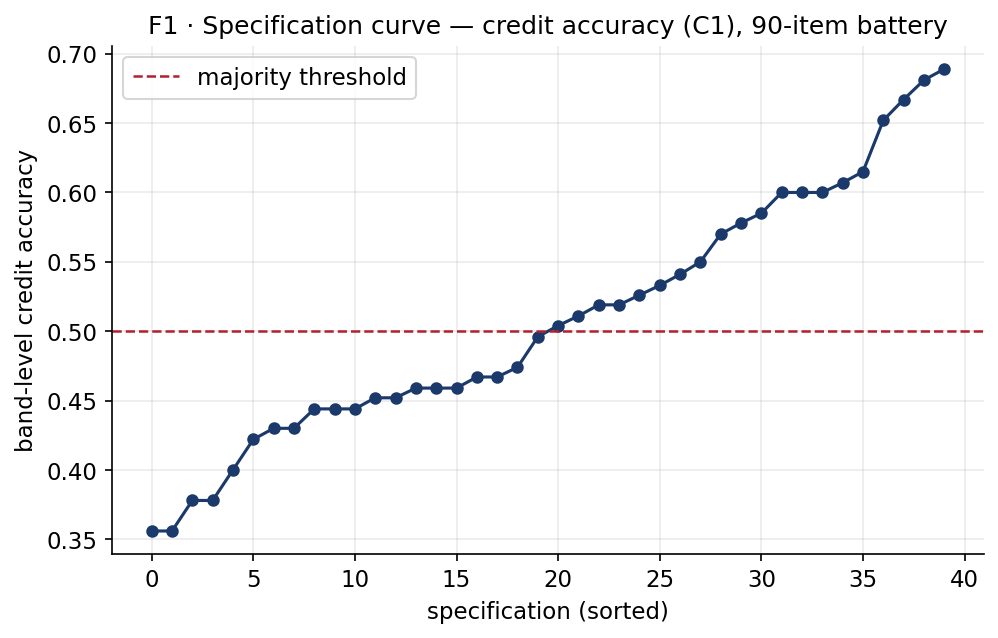
\includegraphics[width=0.82\textwidth]{fig_spec_curve.png}
\caption{Specification curve of the machine credit rating. Each point is one of the pre-registered
specifications (three seeds pooled), ordered by majority-correct credit-band accuracy against the
Altman Z$''$ benchmark. Accuracy ranges widely across specifications despite identical firm
fundamentals, and roughly half reverse the pre-registered accuracy verdict (spec-curve flip share
$\approx0.50$)---the multiverse the method is named for.}
\label{fig:speccurve}
\end{figure}

\begin{table}[t]\centering
\caption{Variance shares of the machine credit letter-rank (mixed-effects). Every controllable design
choice is small relative to run-to-run noise.}\label{tab:var}
\begin{tabular}{lr}\toprule
Component & Variance share \\\midrule
Item (firm profile) & $\sim$63\% \\
Residual seed (run-to-run noise) & $\sim$25\% \\
Answer presentation ($A_7$, largest design axis) & $\sim$5.0\% \\
Provider $\times$ item interaction & $\sim$2.2\% \\
Model provider ($A_1$, main effect) & $\sim$1.3\% \\\bottomrule
\end{tabular}\end{table}

\subsection{Determinism does not save you}
The natural rebuttal is that the noise floor is an artifact---two of the three providers ignore
temperature $=0$, so residual run-to-run variation might vanish under genuine determinism. We pre-registered
the test. Restricting to the one provider$\times$setting whose metadata confirms honored determinism
(Google at temperature 0), the fragility does not vanish: across deterministic prompt configurations,
majority-correct credit-band accuracy still ranges 0.36--0.69, and 62.5\% of specifications flip the
majority verdict, with a permutation test decisively rejecting specification-invariance (no permuted
labeling exceeded the observed statistic; $p=(k{+}1)/(n{+}1)=0.001$ over 999 permutations). Determinism
removes run-to-run jitter but leaves specification fragility intact---the flip share inside the
deterministic subgrid is higher, not lower, than the pooled estimate.

\subsection{No vendor escape}
The $\sim$1.3\% provider main effect sits beside a fact that seems to contradict it. Across the two
families at full snapshot coverage (OpenAI and Google; xAI contributes its current snapshot only, its
prior snapshot being a documented dead cell), on identical firms across seeds, within-vendor agreement
exceeds cross-vendor agreement at every granularity: 73.7\% within versus 50.4\% across at the band
level, 22.5\% versus 5.2\% at the letter level. Both hold, and together they close both exits. Provider
is a negligible \emph{level} effect but enters through a large provider$\times$item interaction:
vendors disagree, but idiosyncratically, name by name, not as a constant shift a desk could calibrate
out---unlike the persistent, characterizable differences of opinion documented among human rating
agencies \cite{cantorpacker1997}. Switching vendors does not reliably change the rating on a given
name, and pooling vendors does not eliminate the observed specification instability.

\subsection{A rating that will not hold a notch---or the investment-grade line}
Because the credit view is elicited at full letter resolution (AAA\ldots C) and coarsened
deterministically, we can ask the sharpest form of the question: at what rating granularity does the
opinion become reproducible across specifications? It never fully does. Raw cross-specification
agreement rises with coarseness but never clears 80\%---16\% at the letter grade, 34\% at the notch,
65\% at the three-way band, and 73\% even at the two-way IG/HY split (equivalently, the disagreement
shares plotted in Fig.~\ref{fig:ighy}). Chance-corrected, Fleiss' $\kappa$
tops out at 0.46 (IG/HY) and falls to 0.39, 0.18, and 0.08 at finer scales; no granularity reaches the
$\kappa=0.6$ conventionally required for substantial agreement (Fig.~\ref{fig:kappa}). This is not a
model hedging to one central grade: all 21 letter grades are used, with scale-usage entropy 4.03 of a
possible 4.39 bits. The opinion is fully expressed and genuinely unstable, not compressed. The priced
information that notch-level distinctions carry \cite{kligersarig2000,tang2009} therefore cannot be
reliably delivered by a machine rater elicited this way.

\subsection{What it costs: turnover, spreads, and capital}
The stability question becomes a markets question at the boundary. We define the per-comparison flip
rate as follows: for each firm profile we draw two of its elicitations uniformly at random from the full
grid---so that the two draws may differ on any elicitation axis (provider, model version, temperature,
prompt paraphrase, output format, few-shot exemplars, answer presentation) and on the random seed, with
no axis held fixed---and record whether they fall on opposite sides of the IG/HY line; the reported rate
is the mean of this per-firm flip probability (one minus the Gini--Simpson concentration of the firm's
IG/HY labels). On this measure, 26.8\% (95\% CI 20.9--32.5\%) of matched elicitation pairs move a name
across the IG/HY boundary. A desk
mechanically following the modal call would incur 56.8\% (95\% CI 50.9--62.7\%) turnover attributable
purely to elicitation choices; the effect remains economically large even at the lower bound of each interval.
Anchored to the Cornaggia et al.\ rating-spread schedule (80--140 bps per 2--3 notches)
\cite{cornaggia2018}, the within-name spread range has a median near 860 bps, inflated by CCC
saturation; for non-saturating names the median range is $\sim$261 bps, never below $\sim$106 bps. And
in regulatory-capital units---mapping each specification's ratings through the Basel standardized
approach \cite{bcbs2019cre20} as a labeled post-hoc cut---the \emph{same} \$45bn equal-weight
corporate book requires between \$2.0bn and \$4.2bn of Pillar-1 minimum capital depending only on how
the rating was requested. As a calibration (not an identity), two randomly chosen specifications differ
on average by \$0.65bn, or 20.5\% of the median---comparable to the $\sim$20\% relative dispersion the
Basel RCAP exercise found across internal-model banks holding identical portfolios
\cite{bcbs2013rcap}. The choice of \emph{how} to ask, not \emph{what} is asked, moves a name by
hundreds of basis points and billions in capital across the most consequential boundary in credit
(Table~\ref{tab:frag}).

\begin{table}[t]\centering
\caption{Fragility in decision and economic units.}\label{tab:frag}
\begin{tabular}{lr}\toprule
Quantity & Result \\\midrule
Specifications flipping majority credit \emph{band} verdict (pooled / determ.) & $\sim$50\% / 62.5\% \\
Credit-band accuracy range, honored-determinism subgrid & 0.36--0.69 \\
Permutation test, determinism subgrid & $p=0.001$ \\
Within- vs cross-vendor agreement (band / letter) & 73.7/50.4 $\cdot$ 22.5/5.2 \\
Max chance-corrected agreement (Fleiss $\kappa$, IG/HY) & 0.46 (no scale $\geq0.6$) \\
Per-comparison IG/HY boundary flip & 26.8\% (95\% CI 20.9--32.5\%) \\
Implied turnover (modal-call instability) & 56.8\% (95\% CI 50.9--62.7\%) \\
Implied spread range per name (non-saturating / median) & $\sim$261 / $\sim$860 bps \\
Pillar-1 capital range, same \$45bn book (post-hoc cut) & \$2.0bn -- \$4.2bn \\\bottomrule
\end{tabular}\end{table}

\subsection{Real-firm robustness under a decontamination gate}
A natural objection is that the instability reflects our constructed inputs. But evaluating LLMs on
real issuers is itself contaminated: asked to name the company behind an anonymized financial profile,
Gemini-Flash identifies 22\% of mid-cap issuers from the figures alone, with hits clustered and
reasoning-traced. Naive real-firm evaluation can therefore conflate memorized issuer information with
independent credit judgment. We nonetheless build a decontaminated arm: 31 US mid-cap (\$2--15B)
business-to-business issuers whose latest 10-K discloses a current agency rating (extracted with a
verbatim quotation, permanent SEC URL, and document hash). Each dollar figure is scaled by a per-issuer
factor drawn log-uniform$[0.6,1.7]$---which preserves the financial-ratio structure used by the
benchmark while disrupting exact-figure lookup---and consumer-facing firms are
screened out. A pre-registered fingerprinting gate certifies decontamination at 2.9\% identification.
Rating each firm across a frozen 12-specification grid at three seeds, and re-scoring the constructed
battery on the identical grid, the real-arm WATCH flip-share is 0.226 (95\% CI 0.147--0.308), compared
with 0.318 (95\% CI 0.223--0.406) in the matched battery. The estimated difference is $-0.091$
(95\% CI $-0.213$ to $0.032$) (Table~\ref{tab:realarm}). Although the difference is not statistically
distinguishable from zero, formal equivalence within the pre-registered $\pm0.15$ margin is not
established (two-one-sided-tests $p=0.179$), reflecting limited power in the 16-real/15-battery WATCH
samples. The real-firm arm therefore provides evidence that substantial specification instability
persists in real issuers, while the data are insufficient to establish quantitative equivalence with
the constructed battery; the somewhat lower point estimate is consistent with real WATCH names sitting
farther from band thresholds, not with residual memorization. Model bands match the disclosed agency rating
only 54\% of the time.

\begin{table}[t]\centering
\caption{Real-firm arm: 31 decontaminated business-to-business issuers, agency-rating benchmark.}
\label{tab:realarm}
\begin{tabular}{lr}\toprule
Quantity & Result \\\midrule
Fingerprint identification, naive (exact figures) & 22\% \\
Fingerprint identification, decontaminated (gate) & 2.9\% \\
WATCH-stratum flip-share, real arm & 0.226 (0.147--0.308) \\
WATCH-stratum flip-share, battery (same 12 specs) & 0.318 (0.223--0.406) \\
Difference (real $-$ battery), 95\% CI & $-0.091$ ($-0.213$, $0.032$) \\
Equivalence test (TOST, $\pm0.15$ margin) & $p=0.179$ (not established; underpowered) \\
Interpretation & substantial instability persists; equivalence not established \\
Machine band vs.\ disclosed agency rating (descriptive) & 54\% \\\bottomrule
\end{tabular}\end{table}

\begin{figure}[t]\centering
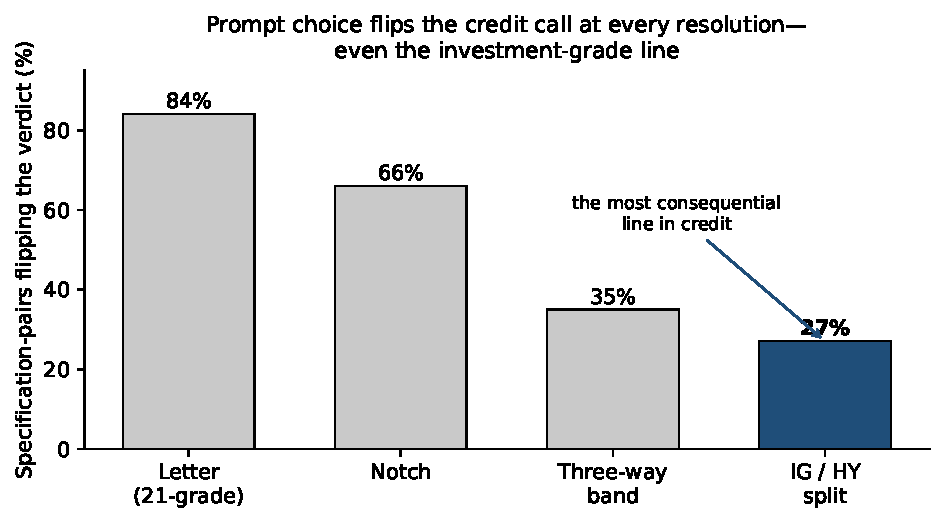
\includegraphics[width=0.66\textwidth]{figure1_ighy.pdf}
\caption{Share of matched elicitation pairs whose credit verdicts differ, by rating granularity, where
the two elicitations of a firm may differ on any grid axis (provider, model version, temperature,
paraphrase, format, few-shot, presentation) and seed. Even at the coarse investment-grade/high-yield
split---the most consequential line in credit---27\% of matched pairs disagree.}\label{fig:ighy}
\end{figure}
\begin{figure}[t]\centering
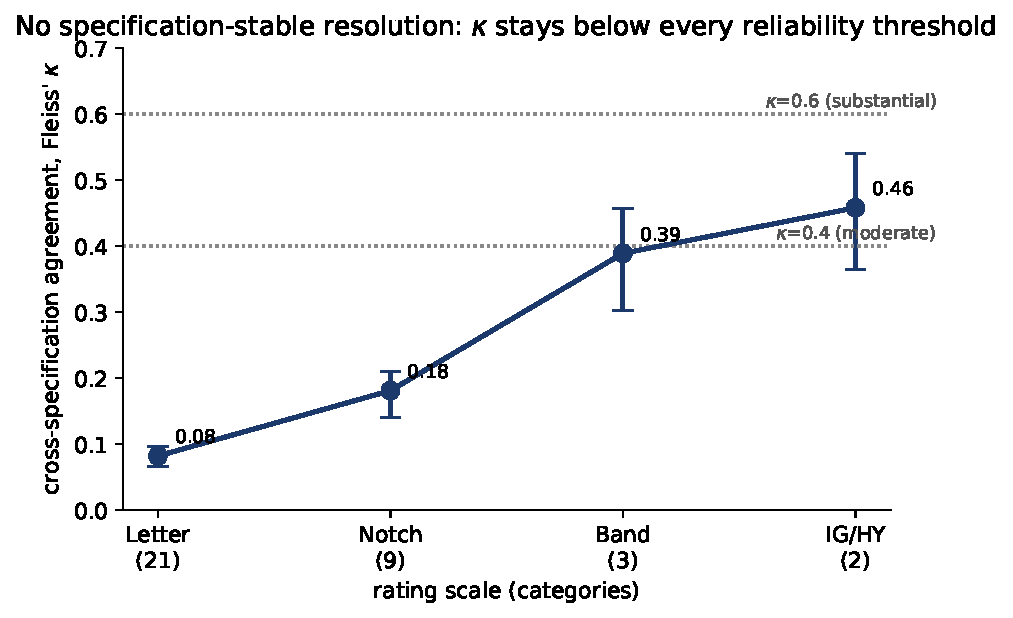
\includegraphics[width=0.62\textwidth]{figureA_kappa.pdf}
\caption{Chance-corrected cross-specification agreement (Fleiss $\kappa$) by granularity; agreement
never reaches the $\kappa=0.6$ substantial-agreement threshold, peaking at 0.46 on the IG/HY split.}
\label{fig:kappa}
\end{figure}

\section{Discussion}
The message for AI-assisted credit is blunt: a single-prompt LLM rating should not be treated as a
specification-invariant measurement, it is one draw from a distribution wide enough to reclassify a firm
across the investment-grade line, to churn a portfolio, and to double a capital charge. The fragility is
dominated by residual run-to-run variation rather than any single elicitation choice a desk could
optimize; it survives honored determinism; it cannot be escaped by switching or pooling vendors; and the
machine credit opinion holds no stable rating resolution, not even the coarse IG/HY split. Critically,
the pattern is not an artifact of synthetic inputs: the qualitative finding of substantial specification
instability extends to real issuers under a design that first \emph{demonstrates} the contamination
of naive real-firm evaluation and then removes it. For a risk function, the practical implication is
that the prompt specification is itself a model-risk parameter under any serious governance standard
\cite{srletter2011}: a rating reported without its specification curve overstates what the model
actually determines. The fingerprinting result is a contribution in its own right---to our knowledge
the first direct evidence that anonymized real-firm LLM evaluation can be contaminated by memorization
even without names in the prompt---and it argues for decontamination gates as standard practice in
financial LLM benchmarking.

\subsection{Limitations}
We make no capability claim: whether these models rate credit \emph{well} is a separate question we do
not adjudicate \cite{drinkall2025forecasting}. The finding is bounded to the three model families and
settings studied, and one prior-version model contributed no data (a documented dead cell). Flip-share
point estimates, though at full power, remain sample statistics on a 90-item battery; the real-firm arm
comprises 31 issuers, thinned to a business-to-business, mid-cap universe by the decontamination screen,
so its strata are smaller than the constructed battery's. The capital and spread translations are
labeled post-hoc calibrations, not pre-registered confirmatory tests. Within those bounds, the stability
conclusion is robust.

\subsection{Future work}
Natural extensions include larger and sector-stratified real-firm samples, retrieval-augmented and
tool-using rating agents, human-in-the-loop workflows that report specification curves rather than point
ratings, and decontamination gates applied to other high-stakes financial LLM tasks.

\section{Conclusion}
Reproducibility in AI-assisted credit cannot be assumed from a single prompt. Across a pre-registered
specification curve, although firm fundamentals explain most rating variation, substantial
specification- and run-level instability remains: the machine credit rating crosses the investment-grade
line for 27\% of matched elicitation pairs; it holds no stable resolution; and the instability survives
determinism, vendor choice, and---under a decontamination gate---the move to real issuers. The
specification is part of the result. A machine rating should be reported, governed, and priced with its
specification curve attached.

\section{Methods}
\textbf{Design rationale.} We use a constructed battery as the primary identification environment
because the estimand is elicitation stability, not performance on a naturally occurring issuer
distribution. The battery holds firm fundamentals fixed, provides a pre-computable objective benchmark,
and permits balanced coverage of credit-health strata while varying only the elicitation specification.
Using real issuers alone would additionally risk contamination from model memorization; we therefore
treat the decontaminated real-firm arm as a complementary external-validity test rather than the
primary identification sample.

\textbf{Battery and benchmark.} The battery is a fixed set of 90 firm-quarter profiles, each carrying a
compact financial statement (revenue, EBIT, total assets and liabilities, equity, working-capital
components, retained earnings). The 90 profiles comprise two equally sized task families: 45
\emph{credit-health} items, on which the model returns a letter/band credit rating, and 45
\emph{directional} items, on which it returns a buy/hold/sell call (used for the turnover translation in
Section~3.5). The credit-rating results and the IG/HY flip rate are computed on the 45 credit-health
items; the directional items enter only the portfolio-turnover measure. For the credit task, each item's
benchmark band is the Altman Z$''$ bond-rating equivalent \cite{altman1968} of its profile (coefficients
6.56/3.26/6.72/1.05; cutoffs 2.60/1.10), with the 45 credit-health items balanced 15/15/15 across the
safe/watch/distress strata. The benchmark was frozen under a pre-registration hash before any model
query; an independent post-hoc re-execution from the frozen facts reproduces all 45 credit-item bands.

\textbf{Specification grid.} Seven researcher-choice axes are crossed: provider (OpenAI, Google, xAI),
model version (a current and a prior snapshot per provider), temperature (0 and 1.0), prompt paraphrase
(three semantically equivalent templates), output format (JSON/free-text), few-shot exemplars (zero or
two), and answer-option presentation (prose/original vs.\ table/reversed). A balance-constrained
D-optimal fraction of 48 specifications was generated (main-effects model, effect-coded; seed frozen),
with a post-hoc parsing-rule axis applied to stored text. Each specification is replicated across three
seeds; the effective temperature returned in provider metadata is logged, because requested temperature
$=0$ is not uniformly honored.

\textbf{Collection.} The full design is 90 items $\times$ 48 specifications $\times$ 3 seeds $=12{,}960$
elicitations; 10{,}793 returned content. One prior-version xAI snapshot returned empty for all 2{,}160
of its cells and is retained as a documented dead cell, not imputed. Each call is stored as an immutable
JSON record; the raw corpus and every downstream stage are fixed by SHA-256 manifests. Collection is
separated from analysis: the confirmatory analysis reads only the frozen response panel and never
re-queries a model.

\textbf{Parsing and statistics.} Stored completions are parsed under three rules (strict, lenient,
tolerant) applied post-hoc; the letter grade is mapped to notch, three-way band, and IG/HY coarsenings.
Agreement is measured by Fleiss' $\kappa$; the contrast between homogeneous and heterogeneous ensembles
by $\Delta\kappa$ with issuer-clustered bootstrap confidence intervals; specification-invariance by a
label permutation test within the honored-determinism subgrid; and variance shares by a mixed-effects
decomposition of the letter-rank with random effects for item, design axes, and their interactions.

\textbf{Statistical analysis.} All analyses are pre-registered unless labelled post-hoc, and inference
uses distribution-free resampling throughout, so no normality assumption is made. Uncertainty on every
headline quantity (the per-comparison IG/HY flip rate, $n=45$ credit-health issuers; implied turnover,
$n=45$ directional issuers; and $\Delta\kappa$) is a percentile bootstrap resampled over issuer clusters
(2{,}000 replicates for the economic quantities, 1{,}000 for the specification-curve quantities), and we
report the point estimate with its two-sided 95\% confidence interval. Specification-invariance is
tested with a one-sided label permutation test on the between-specification spread of band accuracy in
the honored-determinism subgrid (999 permutations; $p=(k{+}1)/(n{+}1)$), the direction being one-sided
because only an excess of observed over permuted spread is evidence against invariance. Equivalence of
the real-firm and battery WATCH flip-shares is assessed by two one-sided tests (TOST) against a
pre-registered $\pm0.15$ margin ($n=16$ real and $15$ battery WATCH issuers). The significance threshold
is $\alpha=0.05$ for all tests. Because a specification curve evaluates many analytic paths, we guard
against selective reporting by pre-registering the estimand and reporting the full curve rather than a
chosen subset; the permutation test is itself a joint (multiplicity-aware) test of the whole grid. We
follow the convention of reserving ``significant'' for results accompanied by a $p$-value and use
``substantial'' or ``considerable'' otherwise.

\textbf{Economic translation (post-hoc).} Rating dispersion is priced by anchoring to the Cornaggia
et al.\ rating-spread schedule and to a cached daily option-adjusted-spread series; portfolio turnover
is the share of names whose modal call changes across specifications. Regulatory capital is computed by
mapping each specification's ratings through the Basel CRE20 external-ratings risk-weight table
(quote-verified) on a \$45bn equal-weight book; the RCAP comparison is a calibration, not an identity.
These translations are labeled post-hoc extensions of the frozen analysis.

\textbf{Real-firm arm.} We identify 31 US mid-cap (\$2--15B) business-to-business issuers whose most
recent 10-K discloses a current long-term agency rating (S\&P primary, else Moody's/Fitch mapped),
extracted with a verbatim quotation, permanent SEC URL, and document hash. To preclude memorization,
every dollar figure is multiplied by a single per-issuer factor drawn log-uniform$[0.6,1.7]$, which
preserves the financial-ratio structure used by the benchmark while disrupting exact-figure lookup;
consumer-facing sectors are screened out. A pre-registered fingerprinting gate probes whether either
model can name the issuer from the anonymized profile; the sample passes at 2.9\% identification
($<5\%$ threshold). Each firm is rated across a frozen 12-specification grid (presentation $\times$
provider $\times$ paraphrase $\times$ format) at three seeds, and the constructed battery is re-scored
on the identical grid for a matched comparison on the WATCH stratum.

\textbf{Reproducibility.} The frozen battery, specification grid, response corpus (12{,}960 records),
analysis code, and manifest hashes are archived; every confirmatory result regenerates byte-for-byte
from the raw corpus through a single offline entry point, with no model calls.

\textbf{Use of generative AI.} Generative AI was used to assist with grammar correction and minor
language edits of the authors' own text, and with software scaffolding, development, and coding of the
analysis and reproducibility pipeline (Anthropic Claude), in all cases under the authors' direction.
Separately, large language models are the object of study in this work---the credit-rating elicitations
under analysis---as described above; every such elicitation is recorded in the specification grid and
frozen corpus. The authors reviewed and verified all such output and take full responsibility for the
content.

\backmatter
\bmhead{Data availability}
All data and code required to reproduce the study are openly available in a deterministic, offline
reproducibility capsule (CodeOcean DOI assigned at deposit; MIT license), mirrored in the source
repository at \url{https://github.com/samirrc2/prompt-choice-credit-ratings}. Within the capsule, the
\texttt{data/frozen/main/} directory contains the pre-registered 90-item firm battery
(\texttt{battery\_90.json}; 45 credit-health $+$ 45 directional items), the specification grid
(\texttt{grid\_definition.json}), the prompt paraphrases (\texttt{paraphrase\_templates.json}), the
rating scale (\texttt{rating\_scale.json}), and the Basel capital map (\texttt{capital\_map.json});
\texttt{data/raw/main/} holds the complete frozen corpus of 12{,}960 model responses;
\texttt{data/panel/panel.parquet} is the analysis panel built once from that corpus; and
\texttt{data/frozen/realarm/} with \texttt{data/raw/realarm/} contain the decontaminated real-firm arm
(the anonymized perturbed battery \texttt{battery\_real45.json}, the sealed issuer crosswalk, the rating
provenance \texttt{ratings\_provenance.csv} with a verbatim 10-K quotation, permanent SEC URL, and
document hash per issuer, and the arm/comparator/fingerprint model-output panels). The analysis code is
in \texttt{analysis/}, pre-computed outputs and figures in \texttt{results/}, and SHA-256 integrity
manifests in \texttt{manifest/}. A single offline entry point, \texttt{reproduce.sh}, regenerates every
reported number, table, and figure byte-for-byte, with no model calls and no API keys. Issuer identities
in the real-firm arm are anonymized and the sealed crosswalk is withheld; the underlying SEC filings
(Form 10-K and company-facts XBRL) are publicly available through the SEC EDGAR system, with permanent
document URLs listed in \texttt{data/frozen/realarm/ratings\_provenance.csv}.

\bmhead{Code availability}
All collection, panel-construction, and analysis code is released under the MIT license in the same
repository; a single \texttt{reproduce.sh} regenerates every reported number, table, and figure from the
frozen data offline. Provider API keys are required only to re-collect the corpus (not to reproduce any
result) and are not distributed.

\bibliography{references}

\bmhead{Author contributions}
\textbf{S.C.:} Conceptualization, Methodology, Software, Formal analysis, Data curation, Writing --
original draft, Writing -- review \& editing. \textbf{R.C.:} Conceptualization, Validation, Writing --
review \& editing. All authors reviewed and approved the manuscript.

\bmhead{Ethics declarations}
This study did not involve human participants, human tissue, or animal subjects, and used no personally
identifiable or sensitive personal data; ethical approval was therefore not required. The analysis uses
only synthetic firm profiles, publicly available corporate financial disclosures (SEC filings), and the
authors' own model elicitations.

\bmhead{Additional Information}
\noindent\textbf{Competing interests:} The authors declare no competing interests.\\
\textbf{Funding:} This research received no external funding.
\end{document}
